\section{Thí nghiệm 2: Thay đổi cấu trúc mạng} 
\label{sec:sim}

Trong môi trường thực tế, mạng cảm biến không dây thường xuyên đối mặt với các thay đổi về cấu trúc do nhiều nguyên nhân khác nhau như thiết bị di chuyển, thiết bị mới được thêm vào, hoặc thiết bị hết pin và rời khỏi mạng. Khả năng thích ứng với những thay đổi này là yếu tố quan trọng quyết định tính ổn định và độ tin cậy của hệ thống. Thí nghiệm này được thiết kế để đánh giá khả năng tự phục hồi và cập nhật định tuyến của thuật toán Gradient khi cấu trúc mạng thay đổi động. Ba kịch bản chính được khảo sát bao gồm: các node trong mạng thay đổi vị trí dẫn đến thay đổi neighbor, node mới tham gia vào mạng đang hoạt động, và node rời khỏi mạng do hết pin hoặc bị tắt. Mục tiêu là kiểm chứng rằng thuật toán có thể tự động cập nhật gradient và bảng định tuyến để duy trì khả năng truyền dữ liệu về sink mà không cần can thiệp thủ công từ người quản trị.

\subsection{Các node trong mạng thay đổi vị trí}
\begin{figure}[h!]
    \centering
    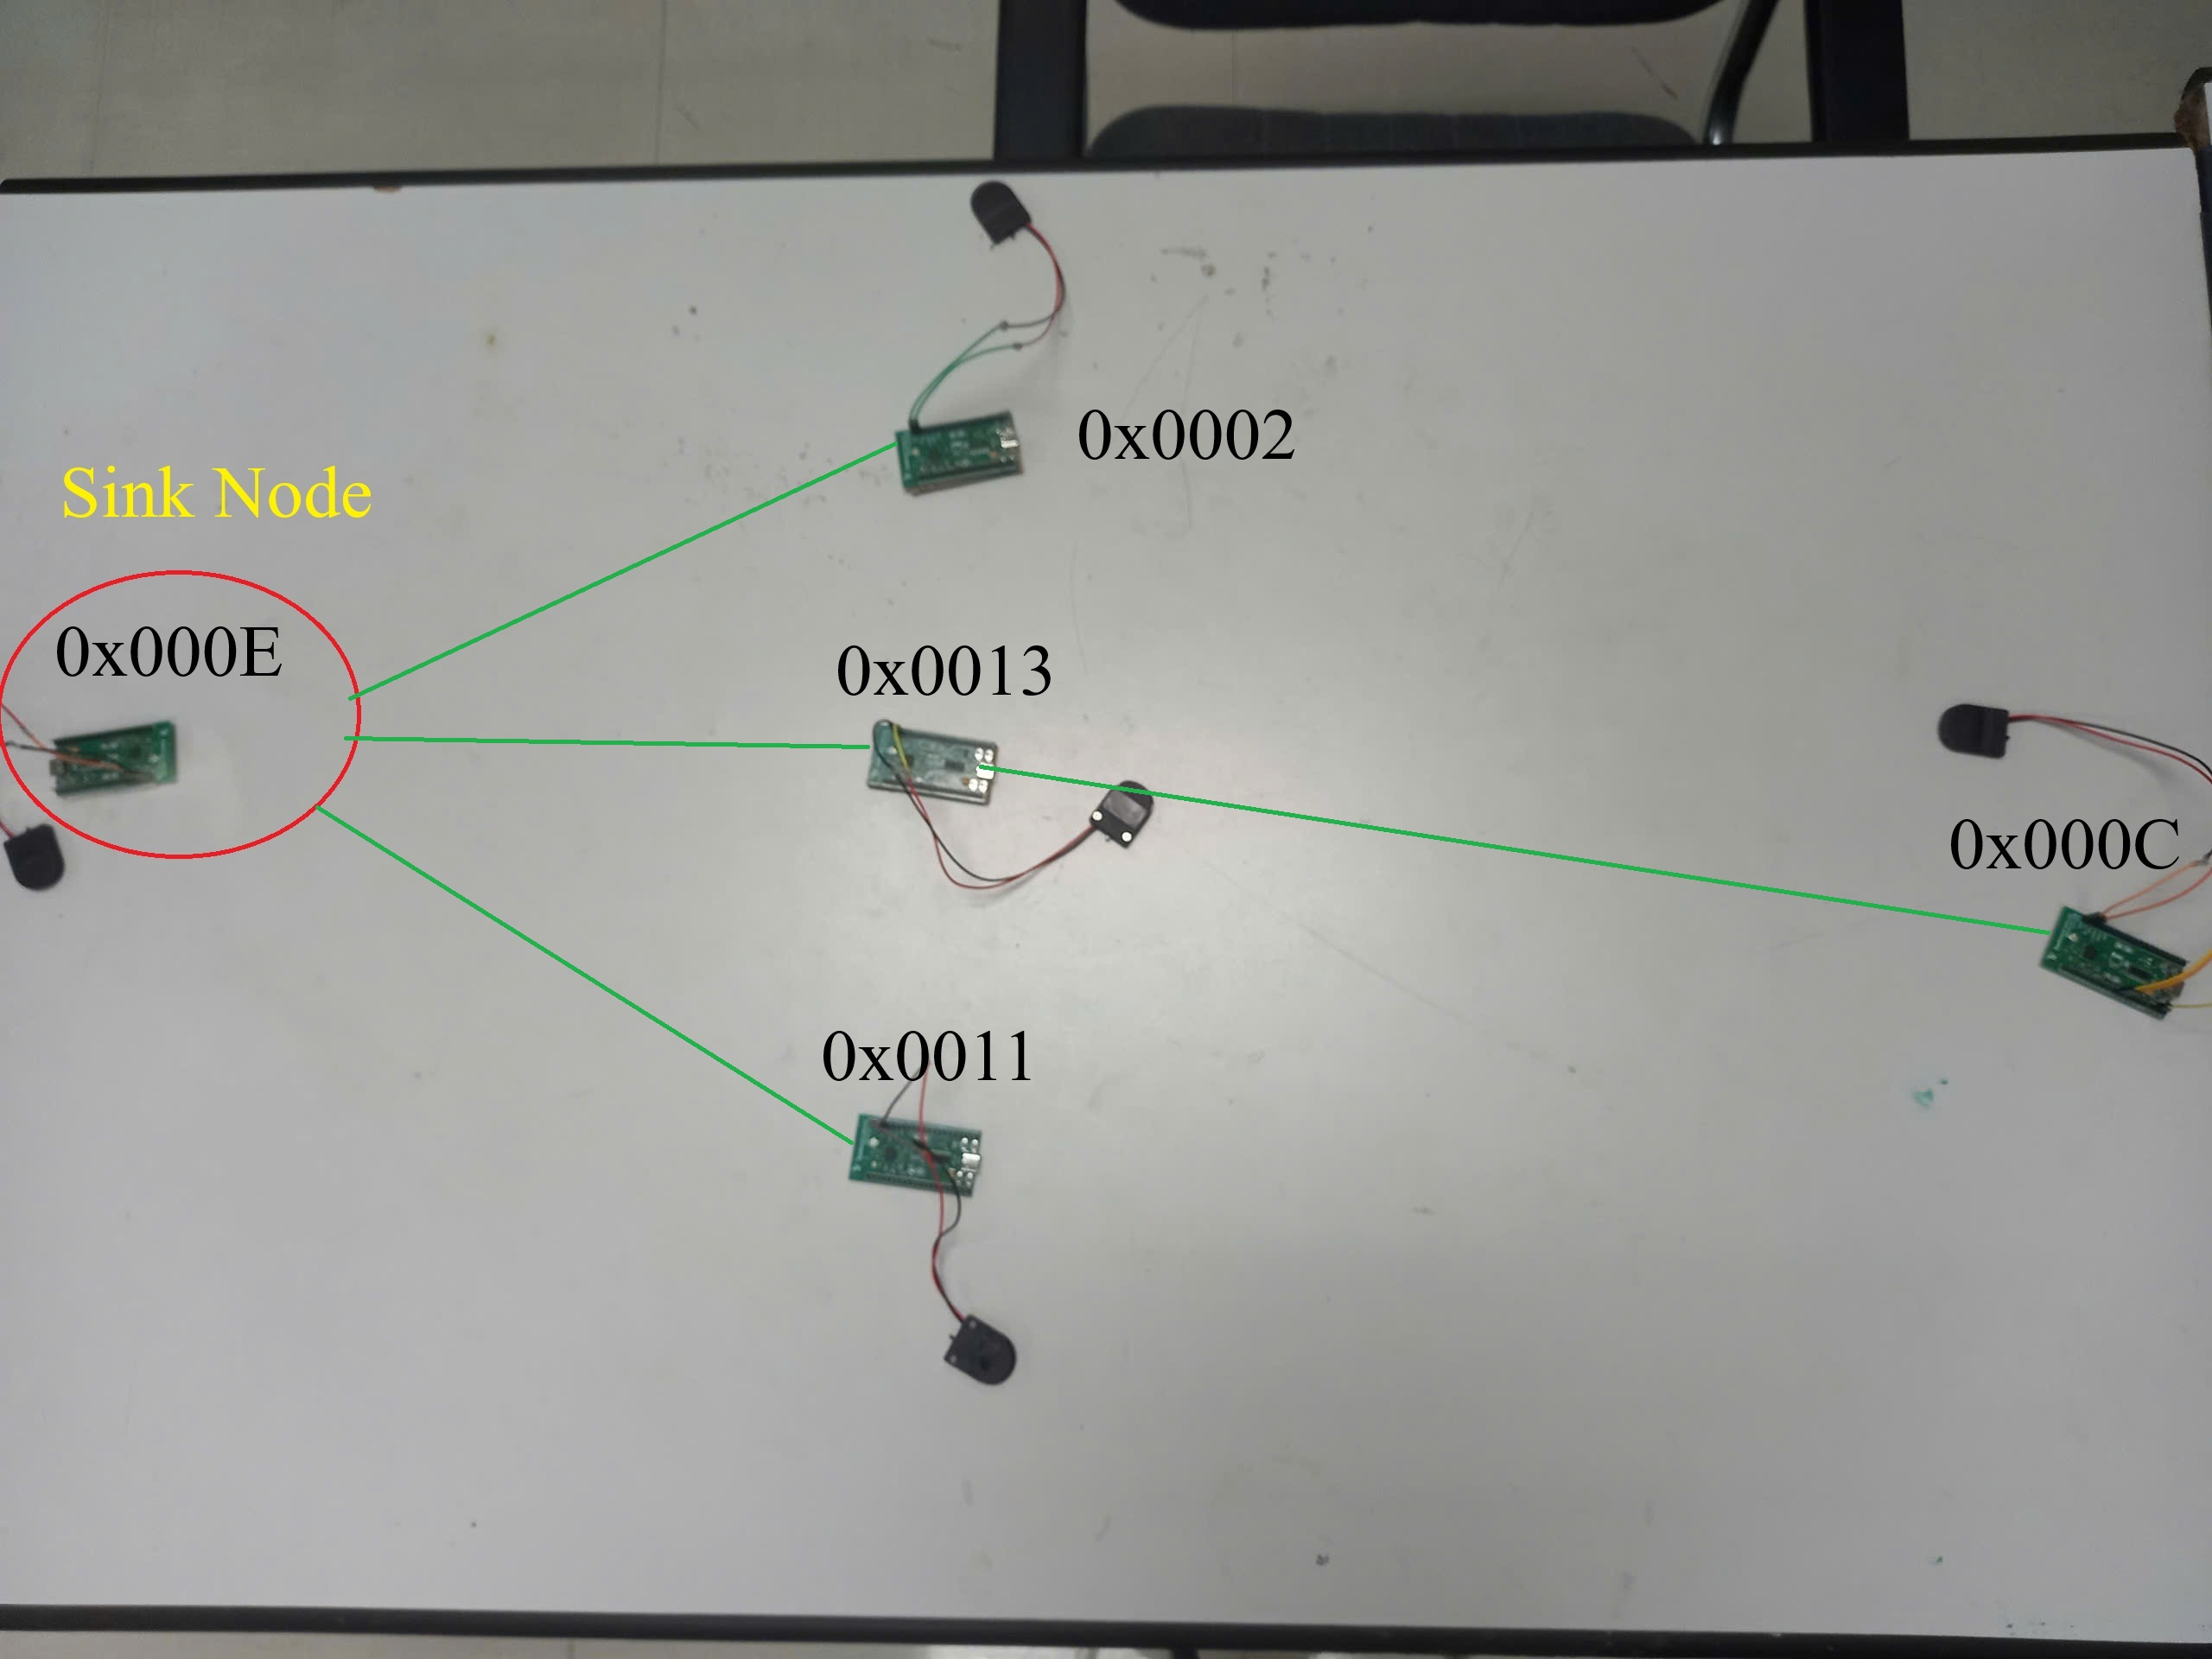
\includegraphics[width=0.48\textwidth]{chapter2/image/demo3_first.jpg}
    \hfill
    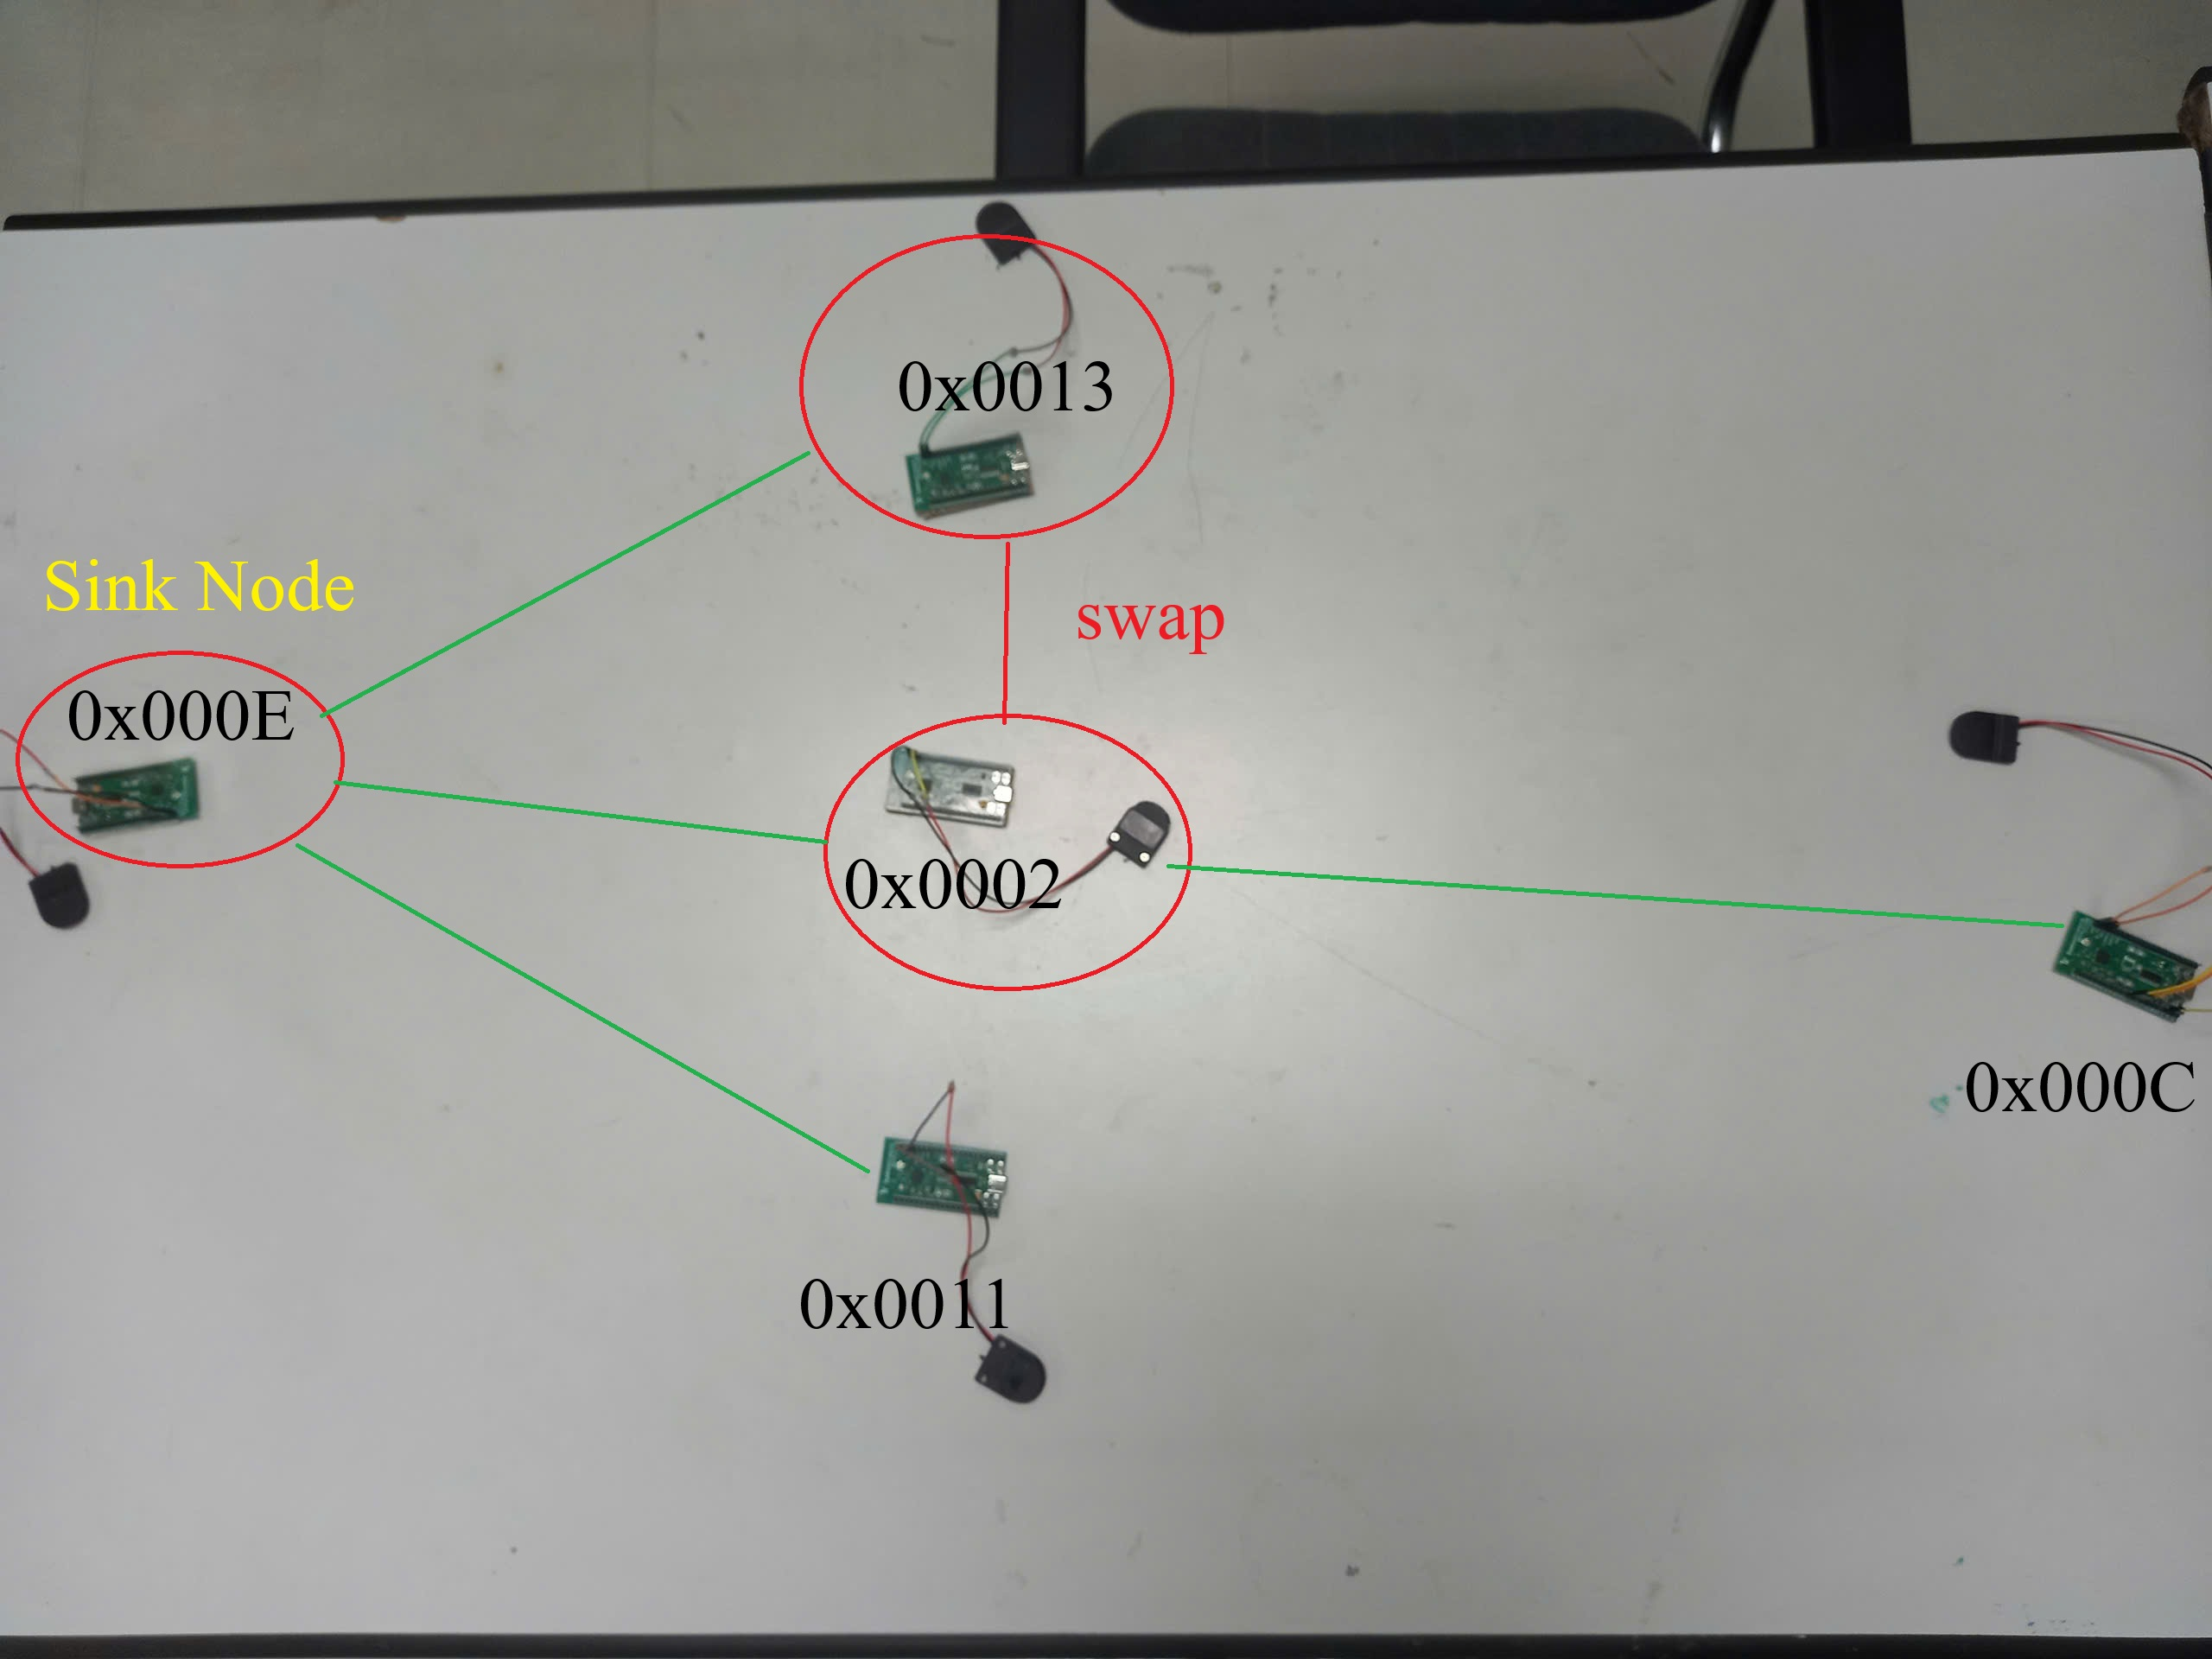
\includegraphics[width=0.48\textwidth]{chapter2/image/demo3_after_swap.jpg}
    \caption{Topology mạng thí nghiệm trước (bên trái) và sau (bên phải) khi thay đổi vị trí node 0x0013 và 0x0002}
    \label{fig:swap_topology}
\end{figure}

Ban đầu mạng được bố trí theo topology như hình bên trái, sau đó ta tiến hành check log để xác nhận tất cả các node đã thiết lập gradient và bảng định tuyến đúng. Tiếp theo, ta thay đổi vị trí của hai node 0x0013 và 0x0002 như hình bên phải, dẫn đến việc RSSI giữa các node khi node 0x000C thu được sẽ thay đổi. Tiến hành check log trên node 0x000C để kiểm tra bảng định tuyến sau khi quá trình thiết lập gradient hoàn tất lại. Kết quả hiển thị trong Hình\ref{fig:swap_topology_routing_table}.

\begin{figure}[h!]
    \centering
    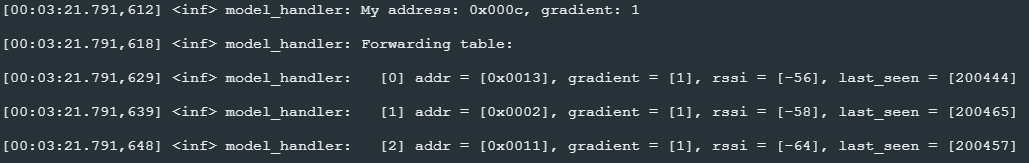
\includegraphics[width=0.75\textwidth]{chapter2/image/0x000C_first.png}
    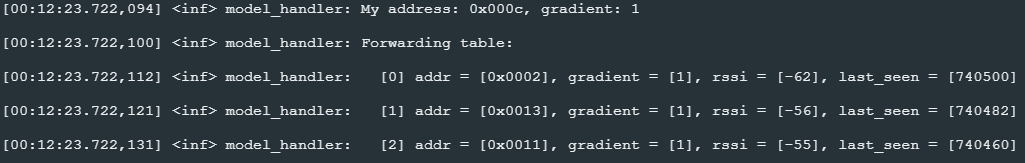
\includegraphics[width=0.75\textwidth]{chapter2/image/0x000C_after_swap.png}
    \caption{Bảng định tuyến của node 0x000C trước (bên trên) và sau (bên dưới) khi thay đổi vị trí node 0x0013 và 0x0002}
    \label{fig:swap_topology_routing_table}
\end{figure}

Từ hình trên, ta thấy rằng sau khi thay đổi vị trí của hai node 0x0013 và 0x0002, bảng định tuyến của node 0x000C đã được cập nhật lại. Ban đầu, node 0x000C chọn node 0x0013 làm next-hop do có RSSI tốt hơn so với node 0x0002. Tuy nhiên, sau khi thay đổi vị trí, RSSI từ node 0x0002 đến node 0x000C trở nên tốt hơn, dẫn đến việc node 0x000C cập nhật bảng định tuyến để chọn node 0x0002 làm next-hop thay vì node 0x0013.

Điều này chứng minh rằng thuật toán Gradient có khả năng tự động điều chỉnh bảng định tuyến dựa trên các thay đổi về liên kết giữa các node, đảm bảo rằng dữ liệu luôn được chuyển tiếp qua các đường dẫn tối ưu nhất về sink.

\subsection{Node rời khỏi mạng}
Thí nghiệm tiếp theo được thực hiện để đánh giá khả năng của thuật toán Gradient trong việc xử lý tình huống khi một node rời khỏi mạng. Trong thí nghiệm này, ta sẽ loại bỏ node 0x0011 như trên hình\ref{fig:delete_topology_routing_table} khỏi mạng và quan sát node 0x000C cập nhật bảng của mình.

\begin{figure}[h!]
    \centering
    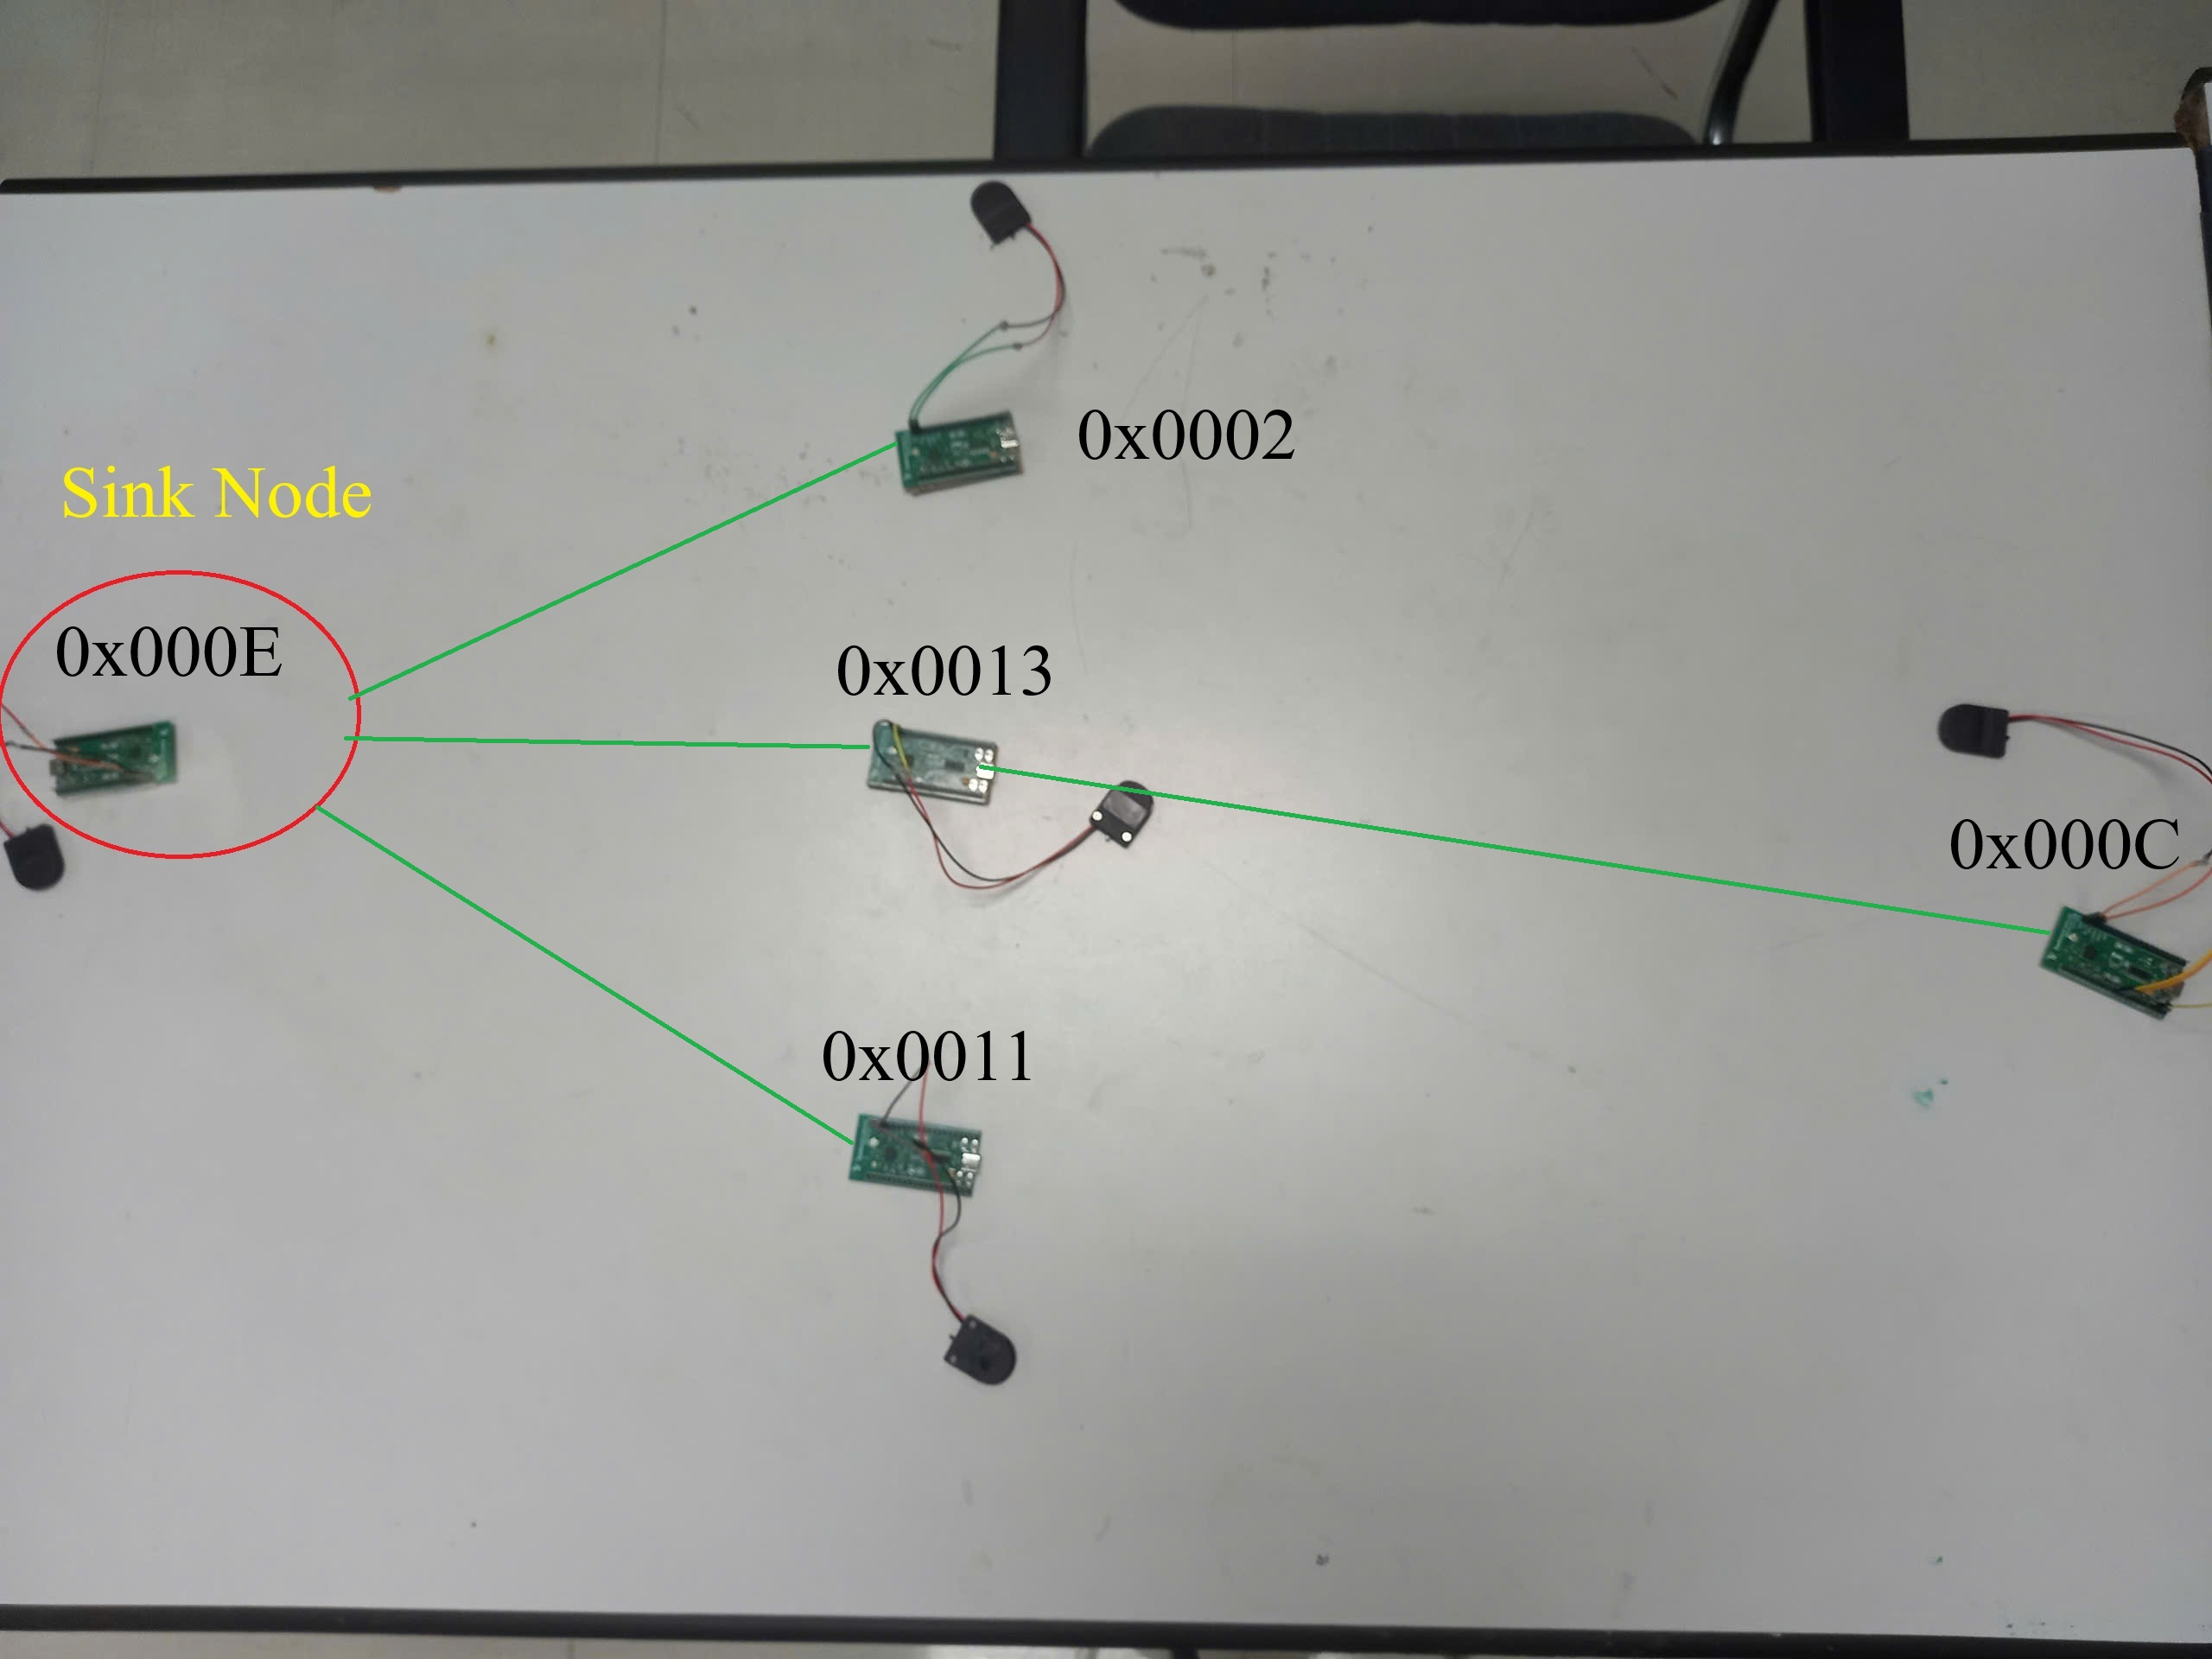
\includegraphics[width=0.48\textwidth]{chapter2/image/demo3_first.jpg}
    \hfill
    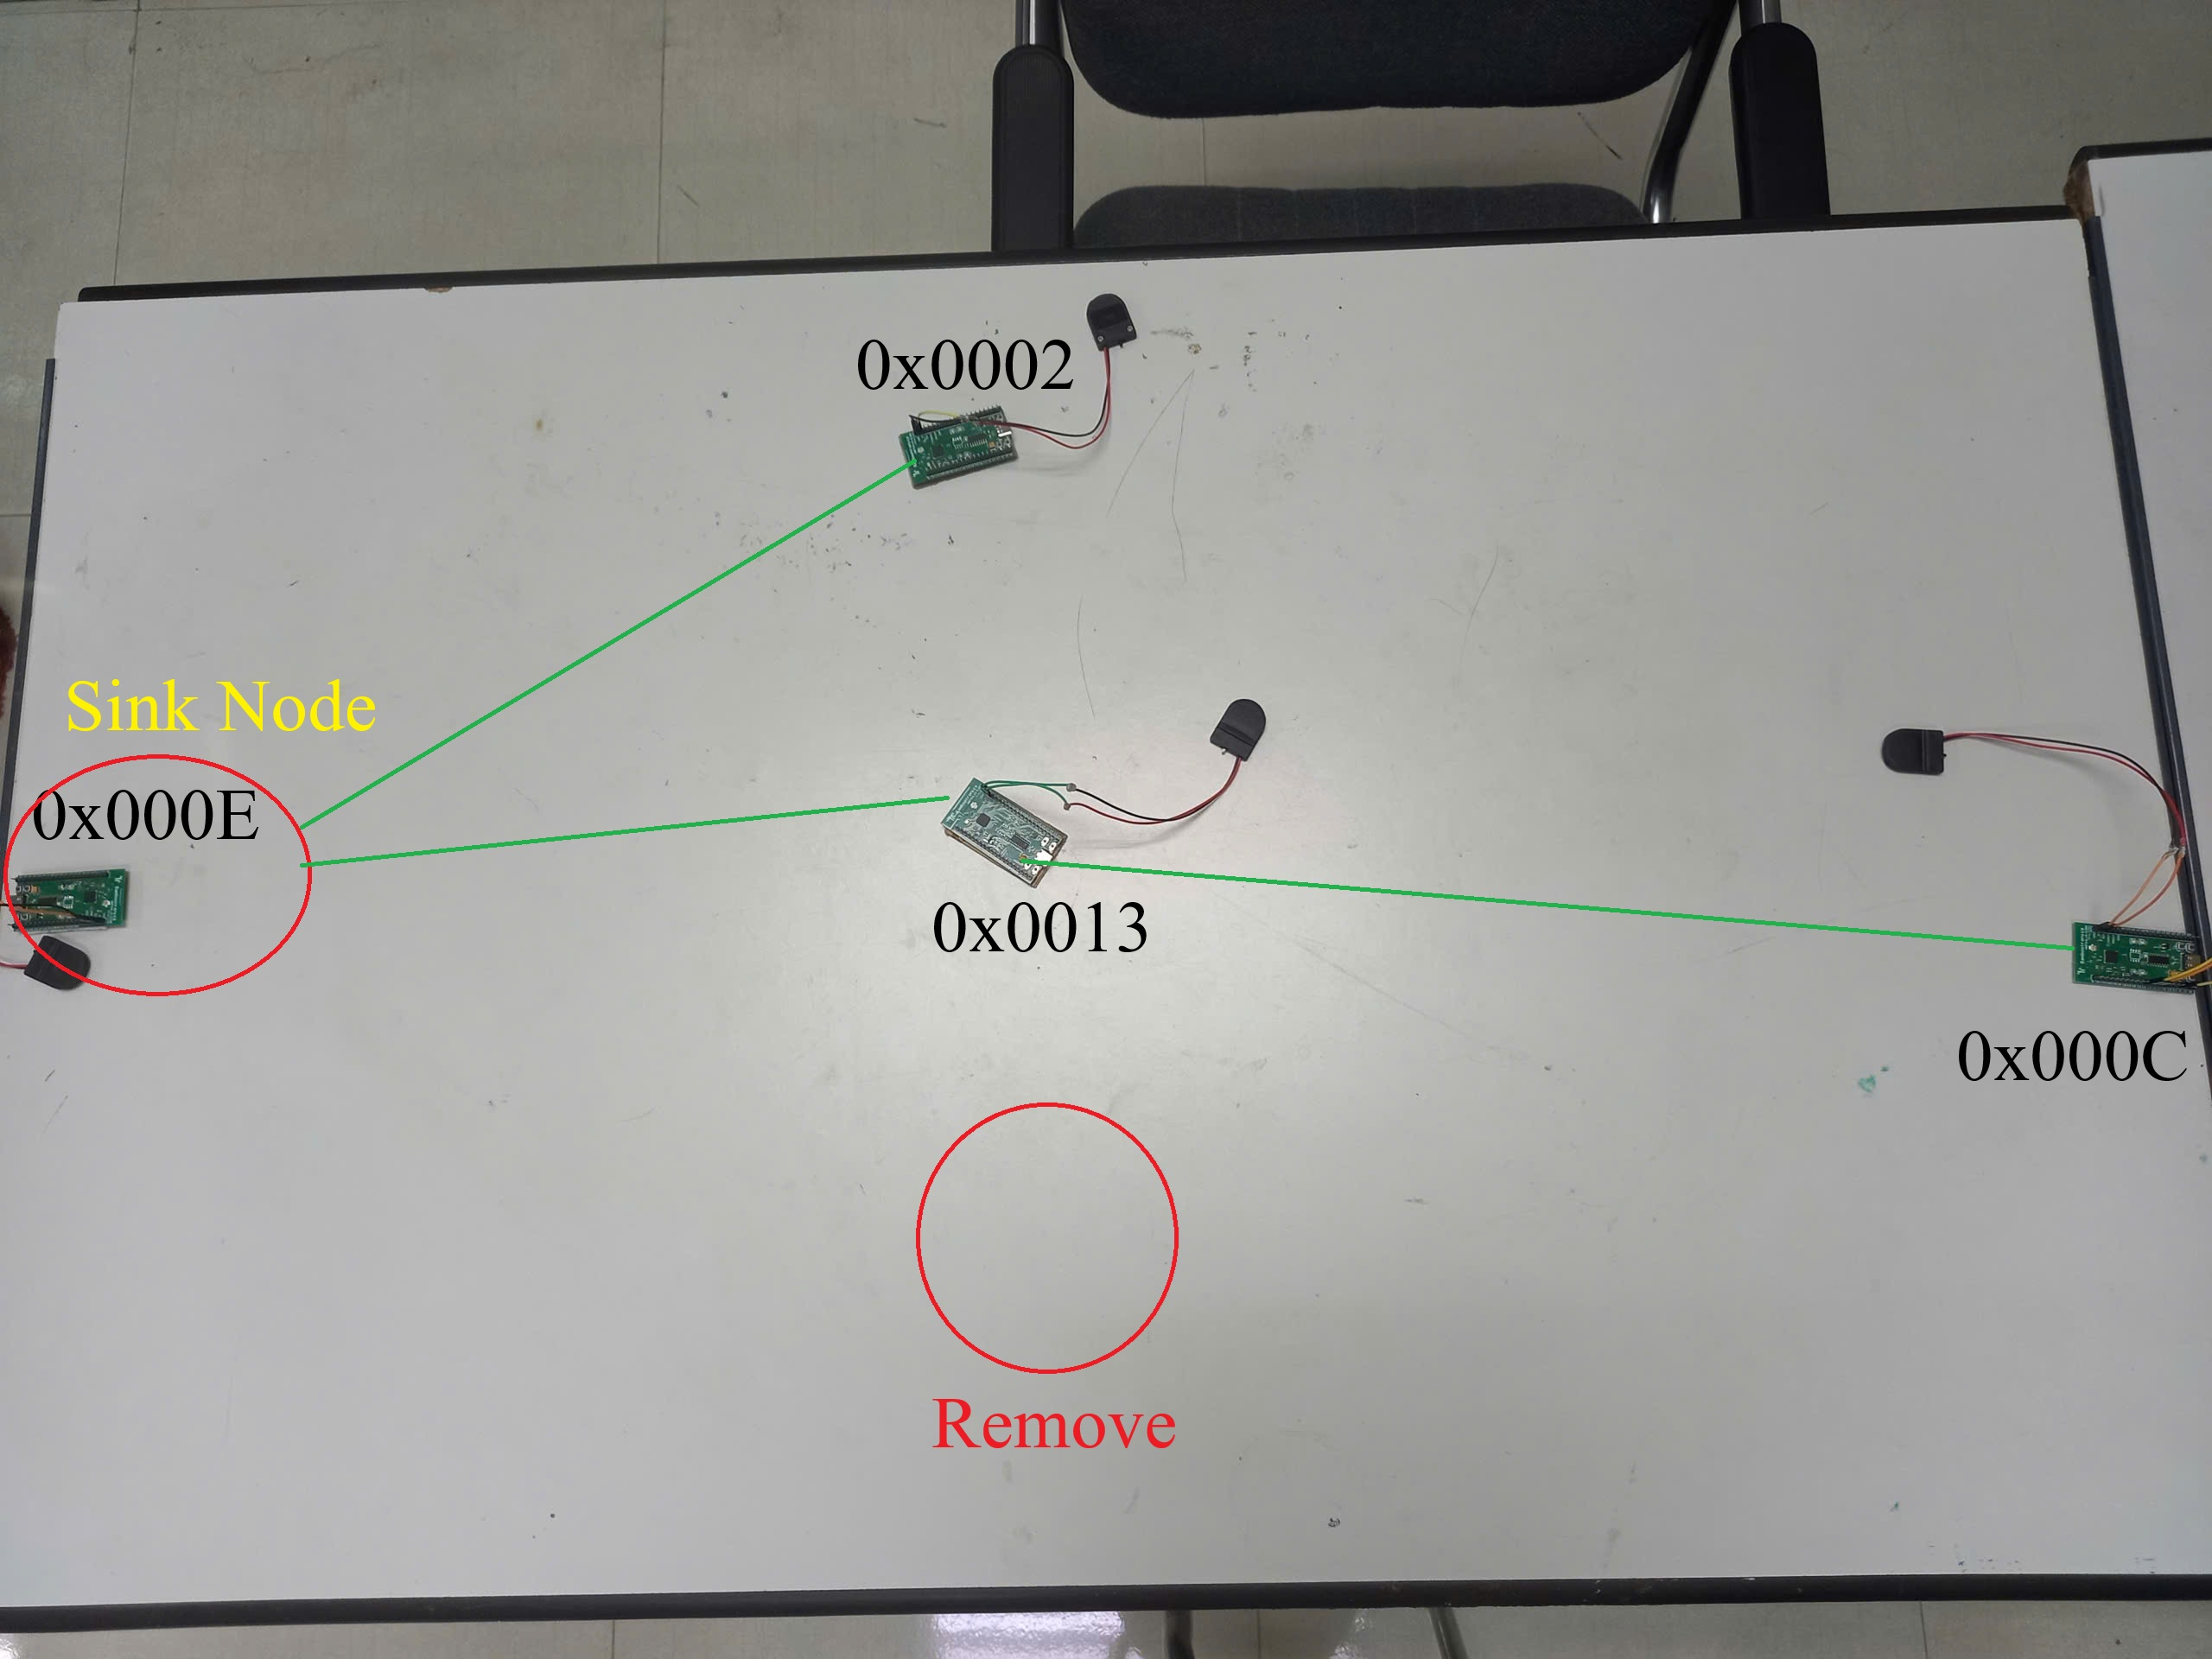
\includegraphics[width=0.48\textwidth]{chapter2/image/demo3_delete.jpg}
    \caption{Cấu trúc mạng trước (bên trái) và sau (bên phải) khi node 0x0011 rời khỏi mạng}
    \label{fig:delete_topology_routing_table}
\end{figure}

Tiến hành check log trên node 0x000C để kiểm tra bảng định tuyến sau khi node 0x0011 rời khỏi mạng. Kết quả hiển thị trong Hình\ref{fig:delete_topology_routing_table_result}.

\begin{figure}[h!]
    \centering
    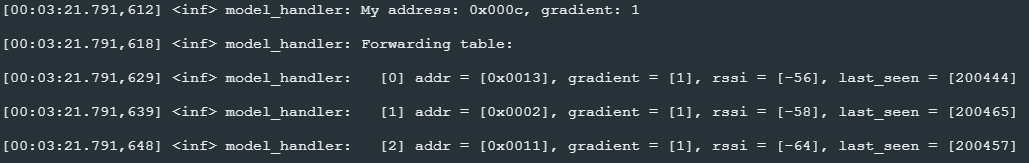
\includegraphics[width=0.75\textwidth]{chapter2/image/0x000C_first.png}
    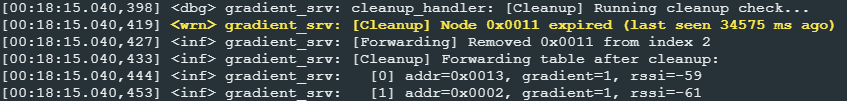
\includegraphics[width=0.75\textwidth]{chapter2/image/0x000C_delete.png}
    \caption{Bảng định tuyến của node 0x000C trước (bên trên) và sau (bên dưới) khi node 0x0011 rời khỏi mạng}
    \label{fig:delete_topology_routing_table_result}
\end{figure}

Ta có thể thấy thông báo node 0x0011 không còn xuất hiện trong thời gian khoảng timeout là 30s, sau đó node 0x000C đã cập nhật bảng định tuyến của mình để loại bỏ node 0x0011 khỏi danh sách next-hop. Điều này chứng minh rằng thuật toán Gradient có khả năng phát hiện và xử lý tình huống khi một node rời khỏi mạng, đảm bảo rằng bảng định tuyến luôn phản ánh đúng trạng thái hiện tại của mạng và duy trì khả năng truyền dữ liệu về sink một cách hiệu quả.

\subsection{Node mới tham gia mạng}

Khi một node mới tham gia vào mạng, các node trong mạng cần cập nhật bảng định tuyến của mình nếu node mới này cung cấp một đường dẫn tốt hơn đến sink. Thí nghiệm này được thực hiện bằng cách thêm một node mới với địa chỉ 0x001D vào mạng đã hoạt động và quan sát cách các node khác cập nhật bảng định tuyến của mình.

\begin{figure}[h!]
    \centering
    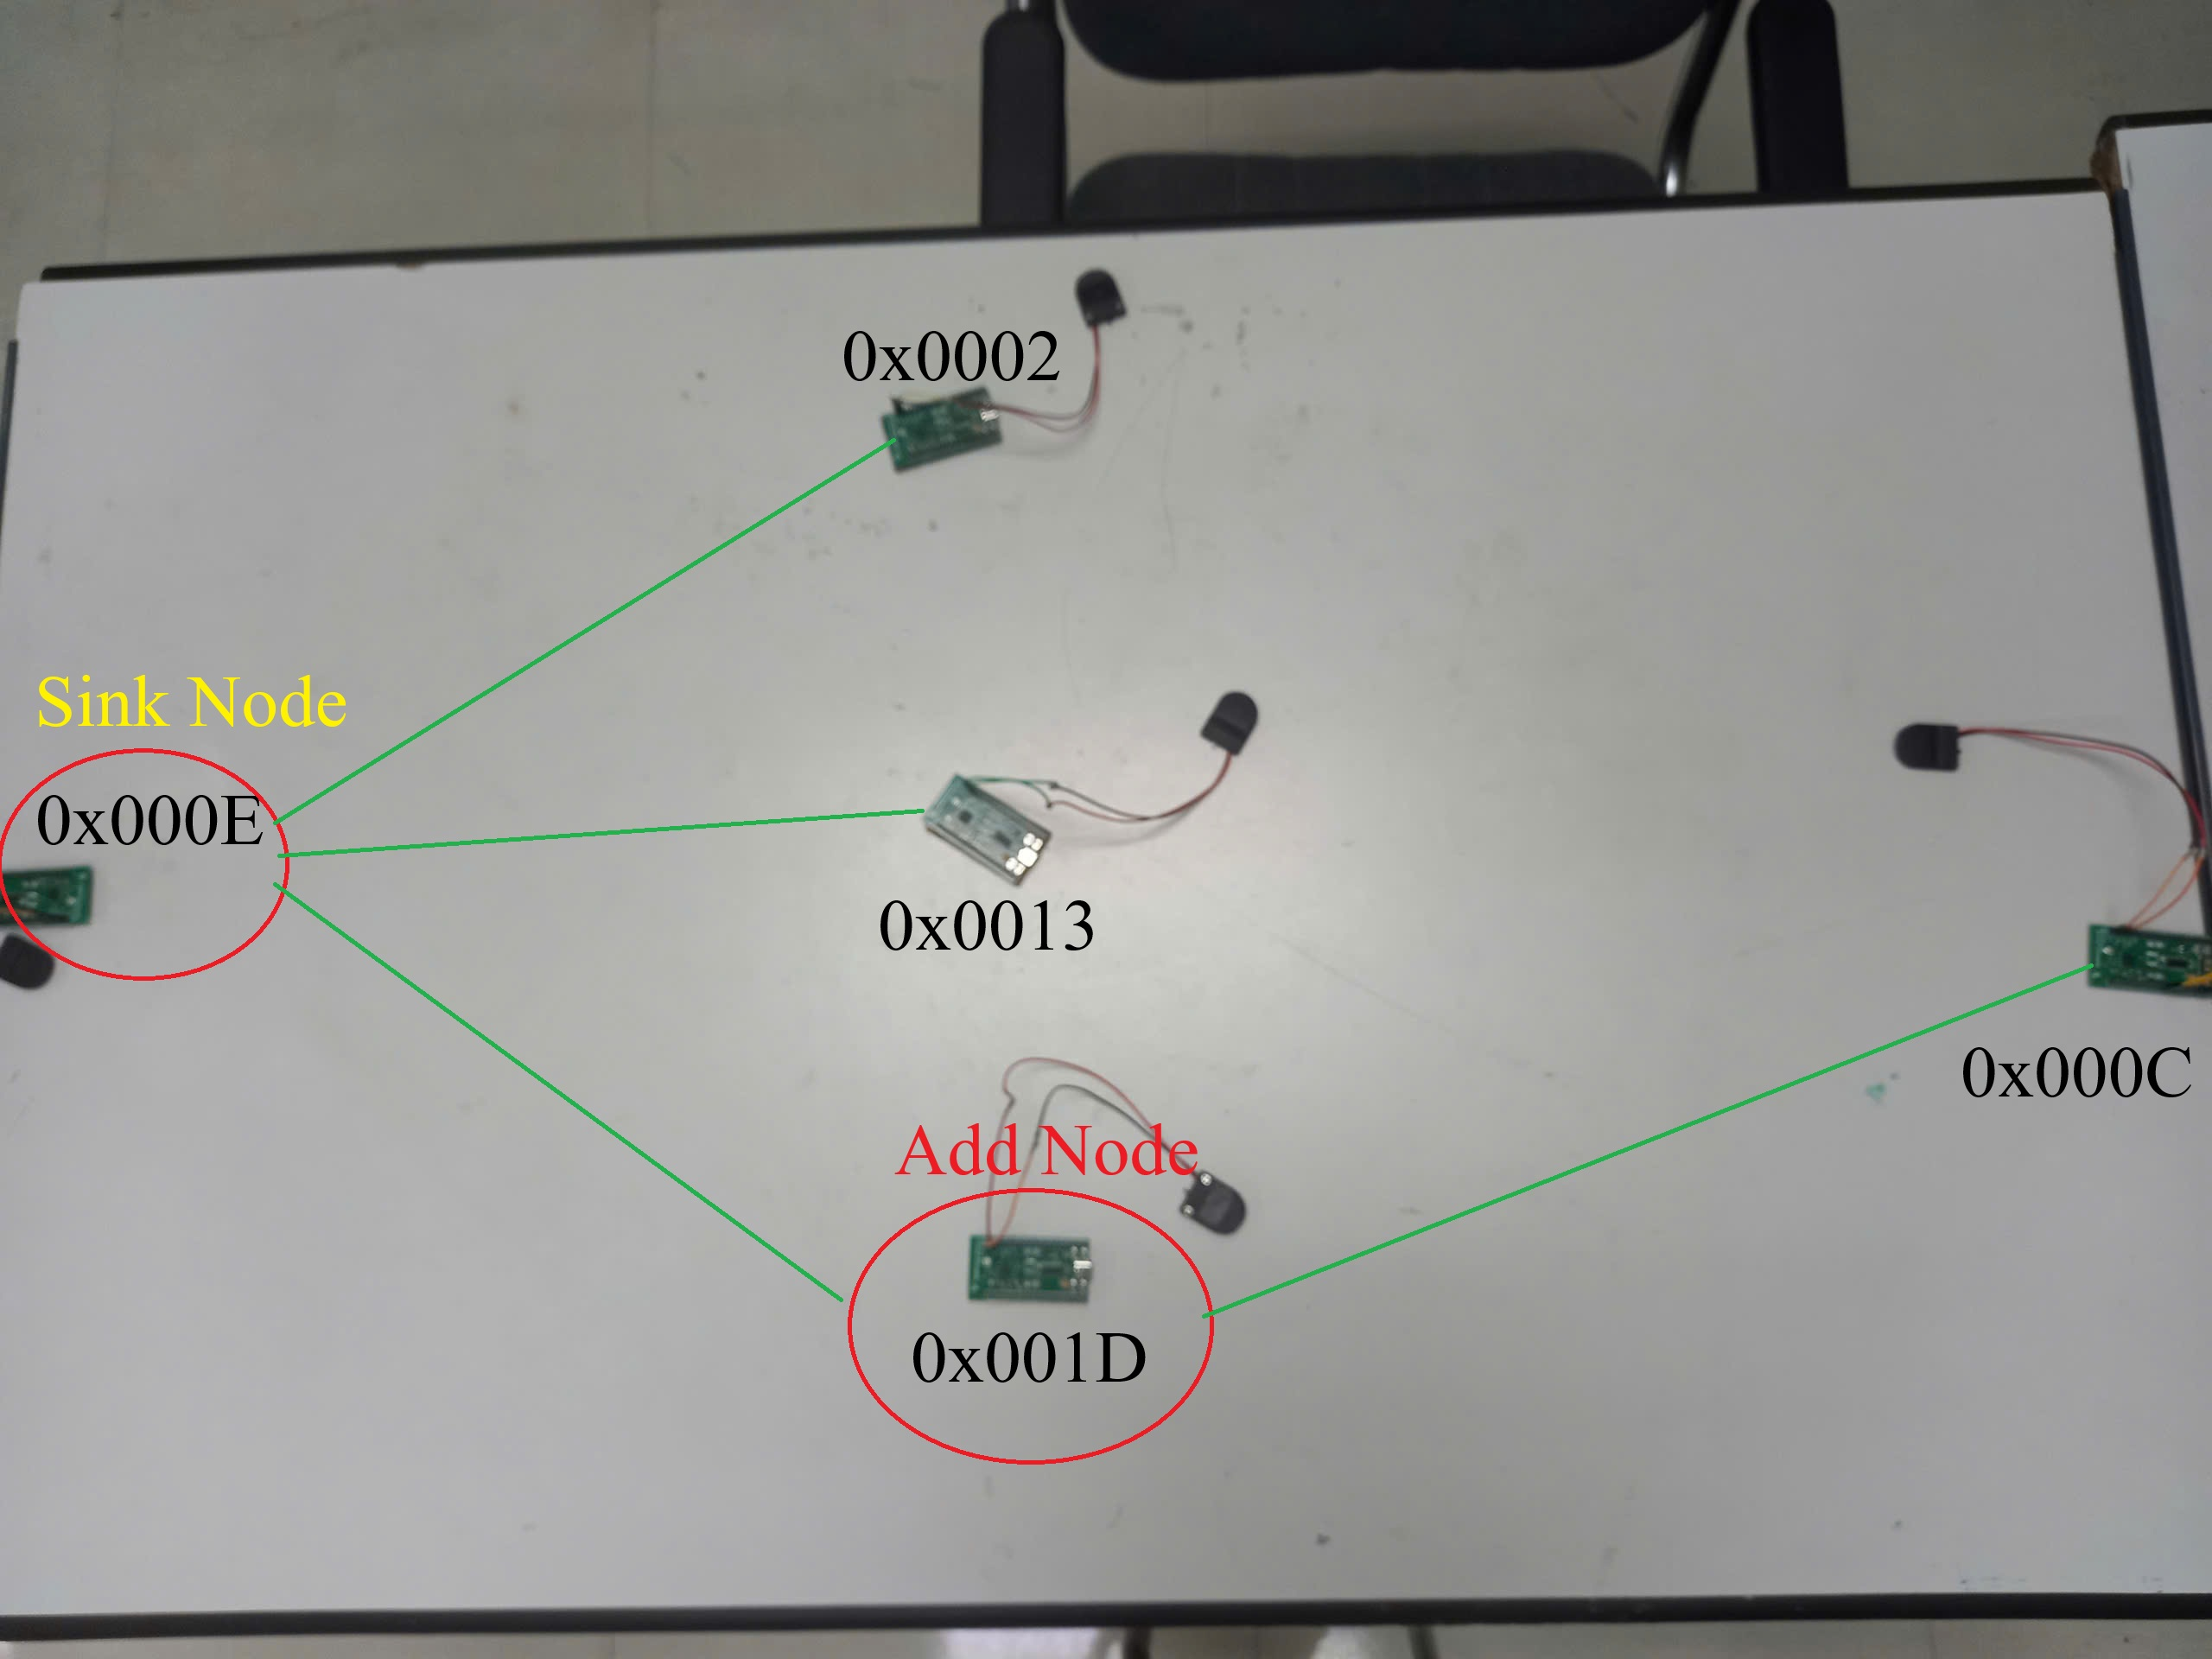
\includegraphics[width=0.75\textwidth]{chapter2/image/demo3_add.jpg}
    \caption{Cấu trúc mạng khi có sự tham gia của node mới 0x001D}
    \label{fig:new_node_topology}
\end{figure}
Tiến hành check log trên node 0x000C để kiểm tra bảng định tuyến sau khi node 0x001D tham gia mạng. Kết quả hiển thị trong Hình\ref{fig:new_node_routing_table}.
\begin{figure}[h!]
    \centering
    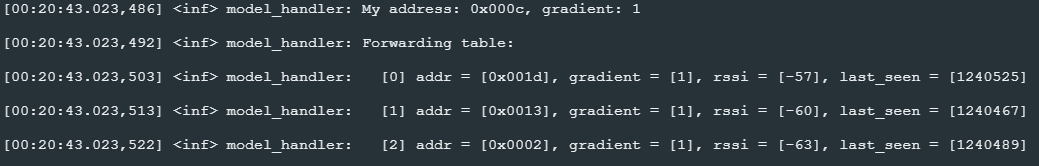
\includegraphics[width=0.75\textwidth]{chapter2/image/0x000C_add_node.png}
    \caption{Bảng định tuyến của node 0x000C khi node 0x001D tham gia mạng}
    \label{fig:new_node_routing_table}
\end{figure}

So sánh bảng định tuyến trong hình \ref{fig:new_node_routing_table} với bảng định tuyến trong hình \ref{fig:delete_topology_routing_table_result} trước đó khi node 0x0011 vừa rời khỏi mạng, ta thấy rằng node 0x000C đã thêm node 0x001D vào bảng định tuyến của mình. Điều này chứng tỏ rằng thuật toán Gradient có khả năng nhận biết sự xuất hiện của node mới và cập nhật bảng định tuyến để tận dụng các đường dẫn tốt hơn đến sink.

